\paragraph{QuizziPedia::Front-End::Directives::MenuBarDirective}
\label{QuizziPedia::Front-End::Directives::MenuBarDirective}

\begin{figure}[ht]
	\centering
	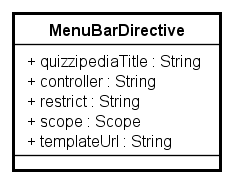
\includegraphics[scale=0.80,keepaspectratio]{UML/Classi/Front-End/QuizziPedia_Front-end_Directives_MenuBarDirective.png}
	\caption{QuizziPedia::Front-End::Directives::MenuBarDirective}
\end{figure} 
\FloatBarrier

\begin{itemize}
	\item \textbf{Descrizione}: rappresenta il menù, presente in ogni pagina dell'applicazione, generato in base agli oggetti passati nello \$scope isolato. Fornisce un pulsante per ogni oggetto ricevuto come parametro, ogni pulsante viene rappresentato con un'icona e con un testo. Al click di un pulsante viene invocata la funzione ad esso associata;
	\item \textbf{Utilizzo}: viene utilizzato per realizzare il menù, presente in ogni pagina dell'applicazione, che permette all'utente di selezionare un'opzione in base al contesto in cui si trova:
		\begin{itemize}
			\item Autenticazione;
			\item Registrazione;
			\item Ricerca;
			\item Visualizzare il proprio profilo utente;
			\item Gestire le domande create;
			\item Gestire i questionari creati.
		\end{itemize}
	\item \textbf{Relazioni con altre classi}: 
	\begin{itemize}
		\item \textbf{OUT \texttt{Index}}: \textit{view\ped{G}} generale dell'applicazione;
		\item \textbf{IN \texttt{MenuBarModelView}}: classe di tipo \textit{modelview\ped{G}} la cui istanziazione è contenuta all'interno della variabile di ambiente \$scope di \textit{Angular\ped{G}}. All'interno di essa sono presenti le variabili e i metodi necessari per il \textit{Two-Way Data-Binding\ped{G}} tra la \textit{view\ped{G}} \texttt{Index} e il \textit{controller\ped{G}} \texttt{MenuBarController};
		\item \textbf{IN \texttt{SearchDirective}}: \textit{directive\ped{G}} che permette di effettuare la ricerca di utenti e questionari;
		\item \textbf{IN \texttt{LoginBarDirective}}: \textit{directive\ped{G}} contenente il componente che permette di effettuare il redirect alla pagina di login;
		\item \textbf{IN \texttt{SignUpBarDirective}}: \textit{directive\ped{G}} contenente il componente che permette di effettuare il redirect alla pagina di registrazione;
		\item \textbf{IN \texttt{UserBarDirective}}: \textit{directive\ped{G}} contenente il componente che permette di effettuare il redirect alla pagina di visualizzazione del profilo utente personale;
		\item \textbf{IN \texttt{ProfileManagementBarDirective}}: \textit{directive\ped{G}} contenente il componente che permette di effettuare il redirect alla pagina di gestione del profilo;
		\item \textbf{IN \texttt{QuestionsManagementBarDirective}}: \textit{directive\ped{G}} contenente il componente che permette di effettuare il redirect alla pagina di gestione delle domande;
		\item \textbf{IN \texttt{LogoutBarDirective}}: \textit{directive\ped{G}} contenente il componente che permette di effettuare il logout;
		\item \textbf{IN \texttt{QuestionnaireManagementBarDirective}}: \textit{directive\ped{G}} contenente il componente che permette di effettuare il redirect alla pagina di gestione dei questionari.
	\end{itemize}
	\item \textbf{Attributi}: 
	\begin{itemize}
		\item \texttt{+ quizzipediaTitle: String} \\ Attributo che viene utilizzato per visualizzare la giusta traduzione della \textit{label\ped{G}} per il titolo e la descrizione dell'applicazione;
		\item \texttt{+ controller: String} \\ Stringa contenente il nome del \textit{controller\ped{G}} della direttiva;
		\item \texttt{+ restrict: String} \\ Stringa che permette di definire le modalità di inserimento della direttiva all'interno della pagina;
		\item \texttt{+ scope: Scope}: oggetto scope interno della direttiva, contiene le funzionalità per gestire i dati presenti all'interno;
		\item \texttt{+ templateUrl: String} \\ Stringa contenente il percorso del file \textit{HTML\ped{G}} che contiene la direttive.
	\end{itemize}
\end{itemize}